\section{Processos Estocásticos}

\begin{frame}[allowframebreaks]
  \frametitle{Processo Estocástico}
  \begin{itemize}
  \item Falamos de variáveis aleatórias i.i.d. $X_1,X_2, \ldots$. Neste contexto, cada uma delas possui a mesma entropia associada.
  \item O que ocorre quando as v.a.s. não são mais independentes? Como podemos lidar com a entropia do processo, neste caso?
  \end{itemize}

  \begin{definition}[Processo Estocástico Estacionário (sentido-estrito)]
  Uma sequência de v.a.s. $X_1, X_2, \ldots, X_n$ é governada por uma distribuição probabilística é dita
  estacionária em sentido estrito se
	\begin{equation}
	p(X_{1:n} = x_{1:n}) = p(X_{1+l:n+l} = x_{1:n})
	\end{equation}  
  para todo $l$, todo $n$ e todo $x_{1:n} \in \mathcal{X}^n$.
  \end{definition}
\end{frame}

\subsection{Markov}
\begin{frame}[allowframebreaks]
  \frametitle{Processo de Markov}

  \begin{definition}[Processo de Markov de primeira ordem]
  Um processo estocástico é um processo de Markov de primeira ordem se
	\begin{equation}
	p(X_{n+1} = x_{n+1} \mid X_{1:n} = x_{1:n}) = p(X_{n+1} = x_{n+1} \mid X_n = x_n)
	\end{equation}
  \end{definition}
  Neste caso, isto significa que $p(x_{1:n}) = p(x_1)p(x_2 \mid x_1) \ldots p(x_n \mid x_{n-1})$.

  Dado o presente, o futuro e o passado são independentes.


  \begin{definition}[Processo de Markov de ordem $m$]
  Um processo estocástico é um processo de Markov de ordem $m$ se
        \begin{eqnarray}
        p(X_{n+1} = x_{n+1} \mid X_{1:n} = x_{1:n}) = \nonumber \\
	p(X_{n+1} = x_{n+1} \mid X_n = x_n, X_{n-1} = x_{n-1}, \ldots , X_{n-m} = x_{n-m})
        \end{eqnarray}
  \end{definition}
  Neste caso, isto significa que $p(x_{1:n}) = p(x_{m+1} \mid x_{m}, x_{m-1}, \ldots, p(x_1)) \ldots p(x_{n-1} \mid x_{n-2}, x_{n-3}, \ldots, x_{n-m-1})  p(x_n \mid x_{n-1}, x_{n-2}, \ldots, x_{n-m})$.

        \begin{figure}[h!]
        \centering
        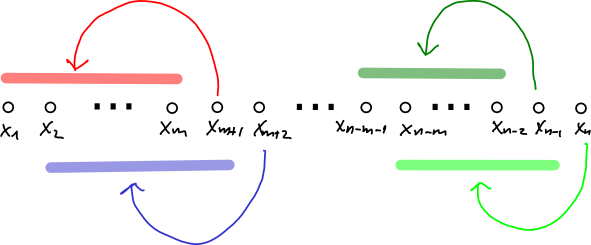
\includegraphics[width=0.8\textwidth]{images/markov-morder.pdf}
        \label{fig:markov-morder}
        \end{figure}

   \framebreak

   \begin{definition}[Homogêneo]
   Uma cadeia de Markov é invariante no tempo (também chamada de homogênea) se $p(x_{n+1} \mid x_n)$ não
   depender do tempo, i.e., se
	\begin{equation}
	p(X_{n+1} = b \mid X_{n} = a) = p(X_2 = b \mid X_1 = a) \quad \forall a,b,n
	\end{equation}   
   \end{definition}
   Neste caso, a cadeia de Markov pode ser descrita por uma matriz de transição fixa $P = [p_{ij}]_{ij}$
   em que $p_{ij} = p(X_{n+1} = j \mid X_{n} = i)$. Podemos representar esta cadeia de Markov como um grafo 
   com setas entre estados cuja probabilidade de transição não é nula.

   \framebreak

   \begin{columns}
   \begin{column}{0.5\textwidth}
	\begin{equation}
	P = \begin{bmatrix}
		0 & p(2 \mid 1) & 0 & p(4 \mid 1) \\
		0 & p(2 \mid 2) & p(3 \mid 2) & 0 \\
		0 & 0 & 0 & p(4 \mid 3) \\
		0 & 0 & 0 & p(4 \mid 4) \\
		\end{bmatrix}
	\end{equation}
   \end{column}
   \begin{column}{0.5\textwidth}
	\begin{figure}[h!]
	\centering
	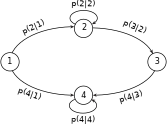
\includegraphics[width=0.6\textwidth]{images/markov-example.pdf}
	\label{fig:markov-example}
	\end{figure}
   \end{column}
   \end{columns}
 
   \begin{itemize}
   \item A probabilidade de um estado no instante $n+1$, dada em função dos possíveis estados no instante $n$ e da probabilidade de transição:
	\begin{equation}
	p(x_{n+1}) = \sum_{x_n} p(x_n) p_{x_n  x_{n+1}}
	\end{equation}
   \item uma cadeia de Markov de primeira ordem é estacionária se $p(x_{n+1}) = p(x_n)$.
   \end{itemize}

   \framebreak

   \begin{definition}[Irredutível]
   Uma cadeia de Markov é irredutível se $p_{ij}(n) > 0$ para todo $i,j$ e para algum $n$ onde
   $p_{ij}(n) = p(X_{n+1} = j \mid X_{n} = i)$.
   \end{definition}
   Ou seja, qualquer estado é acessível de qualquer outro estado (ao menos em algum instante $n$),
   com probabilidade não nula.

   \framebreak

   \begin{definition}[Período]
   Uma cadeia de Markov é periódica se $d(i) > 1$ com
	\begin{equation}
	d(i) = \gcd \{ n : p_{ii}(n) > 0 \}
	\end{equation}
   $d(i)$ é o período do $i$-ésimo estado.
   \end{definition}
   Note que temos o máximo divisor comum do número de épocas para o qual um retorno ao mesmo estado é possível.


   No caso de uma cadeia de Markov homogênea (invariante no tempo), se houver algum $p_{ii} > 0$, 
   o período será $1$ época.

   \framebreak

   \begin{example}
     \begin{columns}
     \begin{column}{0.5\textwidth}
	\begin{equation}
	P = \begin{pmatrix} 1 - \alpha & \alpha \\ \beta & 1 - \beta \end{pmatrix}
	\end{equation}
     \end{column}
     \begin{column}{0.5\textwidth}
        \begin{figure}[h!]
        \centering
        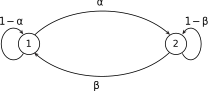
\includegraphics[width=0.6\textwidth]{images/markov-example2.pdf}
        \label{fig:markov-example2}
        \end{figure}
     \end{column}
     \end{columns}

     \begin{itemize}
     \item Se $\mu = [p_1 \ p_2]^T$ é uma distribuição estacionária, então devemos ter $\mu^T P = \mu^T$.
     \item Neste caso, teremos
	\begin{eqnarray}
	\mu^T = \begin{pmatrix} p_1 & p_2 \end{pmatrix} &=& \begin{pmatrix} p_1 & p_2 \end{pmatrix} \begin{pmatrix} 1 - \alpha & \alpha \\ \beta & 1 - \beta \end{pmatrix} \nonumber \\
		&=& \begin{pmatrix} (1-\alpha) p_1 + \beta p_2 & \alpha p_1 + (1-\beta) p_2 \end{pmatrix}
	\end{eqnarray}
     \end{itemize}

	\examplebreak

	Teremos então:
	\begin{equation}
	p_1 = (1-\alpha) p_1 + \beta p_2
	\end{equation}
	logo, $p_1 = \frac{\beta}{\alpha} p_2$
	Sabemos também que devemos ter $p_1 + p_2 = 1$. Por conseguinte, teremos
	\begin{eqnarray}
	p_1 + p_2 &=& 1 \nonumber \\
	\frac{\beta}{\alpha} p_2 + p_2 &=& 1 \nonumber \\
	p_2 &=& \frac{\alpha}{\alpha + \beta}
	\end{eqnarray}

	\examplebreak

	Assim, teremos
	\begin{equation}
	\mu = \begin{pmatrix} \frac{\beta}{\alpha + \beta} \\ \frac{\alpha}{\alpha + \beta} \end{pmatrix}
	\end{equation}
   \end{example}

   \framebreak

   \begin{itemize}
   \item Processo estocástico estacionário: a probabilidade dos estados não muda ao longo do tempo.
   \item Homogêneo: a matriz $P$ de transições não muda ao longo do tempo.
   \item Processo de Markov: futuro e passado são independentes dado o presente (ou então: o passado imediado é suficiente, 
	não sendo relevante o passado distante).
   \item Irredutível: todos estados são acessíveis, eventualmente.
   \item Periódico: máximo divisor comum entre os intervalos em que o retorno a um estado é possível.
   \end{itemize}

\end{frame}


\subsection{Média Cesáro}
\begin{frame}[allowframebreaks]
  \frametitle{Média Cesáro}
  \begin{itemize}
  \item considere a sequência $\{a_n , n \geq 1 \}$
  \item construa a sequência $\{b_n , n \geq 1 \}$, onde $b_n = \frac{1}{n} \sum_{i=1}^n a_i$
  \item $b_n$ é a média Cesáro de $\{a_n\}$
  \end{itemize}

  \begin{lemma}[Média Cesáro]
  Sejam $a_n$ números reais, se $a_n \rightarrow a$ quando $n \rightarrow \infty$ e $b_n = \frac{1}{n} \sum_{i=1}^n a_i$,
  então $b_n \rightarrow a$ quando $n \rightarrow \infty$.
  \end{lemma}  

  \framebreak

  \begin{proof}
  \begin{itemize}
  \item Como $a_n \xrightarrow[ n \rightarrow \infty ]{ } a$, para todo $\epsilon > 0$, existe $N_{\epsilon}$ tal que $\vert a_n - a \vert < \epsilon$
	para todo $n > N_{\epsilon}$.
  \end{itemize}
  \proofbreak
  \begin{itemize}
  \item Para $n > N_{\epsilon}$ teremos
	\begin{eqnarray}
	\vert b_n - a \vert &=& \vert \frac{1}{n} \sum_{i=1}^n a_i - a \vert = \vert \frac{1}{n} \sum_{i=1}^n a_i - \frac{1}{n} \sum_{i=1}^n a \vert \nonumber \\
			&=& \vert \frac{1}{n} \sum_{i=1}^n (a_i - a) \vert  \leq  \frac{1}{n} \sum_{i=1}^n \vert a_i - a \vert \nonumber \\
			&& \text{onde utilizamos a desigualdade triangular} \nonumber \\
			&=& \frac{1}{n} \left( \sum_{i=1}^{N_{\epsilon}} \vert a_i - a \vert + \sum_{i=N_{\epsilon}+1}^n \vert a_i - a \vert \right)
	\end{eqnarray}
  \end{itemize}

  \proofbreak 

	\begin{eqnarray}
        \vert b_n - a \vert &\leq& \frac{1}{n} \left( \sum_{i=1}^{N_{\epsilon}} \vert a_i - a \vert + \sum_{i=N_{\epsilon}+1}^n \vert a_i - a \vert \right) \nonumber \\
		&\leq& \frac{1}{n} \sum_{i=1}^{N_{\epsilon}} \vert a_i - a \vert + \frac{1}{n}  \sum_{i=N_{\epsilon}+1}^n \epsilon \nonumber \\
		&=& \frac{1}{n} \sum_{i=1}^{N_{\epsilon}} \vert a_i - a \vert + \underbrace{\frac{n - N_{\epsilon}}{n}}_{<1} \epsilon 
        \end{eqnarray}

  \proofbreak

        \begin{eqnarray}
	\vert b_n - a \vert &\leq& \frac{1}{n} \sum_{i=1}^{N_{\epsilon}} \vert a_i - a \vert + \underbrace{\frac{n - N_{\epsilon}}{n}}_{<1} \epsilon \nonumber \\
		&<& \underbrace{ \frac{1}{n} \sum_{i=1}^{N_{\epsilon}} \vert a_i - a \vert }_{< \epsilon } + \epsilon < 2\epsilon
	\end{eqnarray}
	onde utilizamos o fato de que podemos tomar $n$ grande suficiente de forma que $\frac{1}{n} \sum_{i=1}^{N_{\epsilon}} \vert a_i - a \vert < \epsilon$,
	pois trata-se de uma soma finita.

	Então $b_n \rightarrow a$ quando $n \rightarrow \infty$.
  \end{proof}

\end{frame}


\subsection{Taxa de Entropia}
\begin{frame}[allowframebreaks]
  \frametitle{Processo Estocástico}
  \begin{itemize}
  \item Processos Estocástico possuem taxas de entropia, que intuitivamente representam o quantidade de 
	informação nova, na média, que é fornecida pelo processo estocástico a cada instante.
  \end{itemize}

  \begin{definition}[Taxa de Entropia de um processo estocástico]
  A taxa de entropia de um processo estocástico $\{ X_i \}_i$ é definida como
	\begin{equation}
	H(\mathcal{X}) \triangleq \lim_{n \rightarrow \infty} \frac{1}{n} H(X_1, X_2, \ldots, X_n)
	\end{equation}
  quando existir.
  \end{definition}
  Note que, quando as v.a.s são i.i.d. teremos % $H(X_1, \ldots, X_n) = H(X_1) + \ldots H(X_n) = n H(X)$ e assim $H(\mathcal{X}) = H(X)$.
  \begin{equation}
	H(\mathcal{X}) = \lim_{n \rightarrow \infty} \frac{1}{n} H(X_{1:n}) = \lim_{n \rightarrow \infty} \frac{1}{n} \sum_{i=1}^n H(X_i) = H(X_1)
  \end{equation}

  A taxa de entropia pode ser vista como a entropia por símbolo para um dado processo estocástico, quando $n$ cresce indefinidamente.

  \framebreak

  \begin{example}
  \begin{itemize}
  \item Se as v.a.s são independentes mas não são identicamente distribuídas, teremos
	\begin{equation}
	\lim_{n \rightarrow \infty} \frac{1}{n} \sum_{i=1}^n H(X_i) = ?
	\end{equation}
	o que pode não existir.
  \end{itemize} 
  \end{example}

 
  \framebreak

  \begin{definition}[Taxa de Inovação da Informação (Definição Alternativa para Taxa de Entropia)]
  Vamos assumir um processo estocástico e definir a taxa da seguinte forma
	\begin{equation}
	H'(\mathcal{X}) \triangleq \lim_{n \rightarrow \infty} H(X_n \mid X_{n-1}, X_{n-2}, \ldots , X_1)
        \end{equation}
  se existir.
  \end{definition}
  Veremos a seguir que $H'(\mathcal{X})$ existe para um processo estocástico estacionário.
 
  \framebreak

  \begin{theorem}
  Para um processo estocástico estacionário, $H(X_n \mid X_{n-1}, X_{n-2}, \ldots , X_1)$ é decrescente com $n$ e possui como limite $H'(\mathcal{X})$.
  \end{theorem}
  \begin{proof}
  \begin{eqnarray}
  H(X_{n+1} \mid X_1, \ldots, X_n) &\leq& H(X_{n+1} \mid X_2, \ldots, X_n) \nonumber \\
		&=& H(X_n | X_1, \ldots, X_{n-1})
  \end{eqnarray}
  Onde utilizamos o fato de que condicionar não aumenta (decresce ou não altera) a entropia; 
  e utilizamos o fato de que o processo estocástico é estacionário.

  Temos então uma sequência decrescente com limite inferior $0$, logo, esta sequência possui um limite: $H'(\mathcal{X})$.
  \end{proof}


  \framebreak

  \begin{theorem}
  Para um processo estocástico estacionários temos
	\begin{eqnarray}
	\lim_{n \rightarrow \infty} H(X_n \mid X_{n-1}, X_{n-2}, \ldots, X_1) \triangleq H'(\mathcal{X}) \nonumber \\
		= H(\mathcal{X}) \triangleq \lim_{n \rightarrow \infty} \frac{1}{n} H(X_1,X_2,\ldots,X_n)
	\end{eqnarray}
  \end{theorem}

  \begin{proof}
	\begin{equation}
	b_n = \frac{H(X_1,X_2,\ldots,X_n)}{n} = \frac{1}{n} \sum_{i=1}^n \underbrace{H(X_i \mid X_{i-1}, \ldots, X_1)}_{=a_i}
	\end{equation}
  como $a_n \rightarrow H'(\mathcal{X})$, teremos $b_n \rightarrow H'(\mathcal{X})$, mas por definição $b_n \rightarrow H(\mathcal{X})$.
  \end{proof}

  \framebreak

  \begin{itemize}
  \item Note que para qualquer processo estacionário ergódico, temos os seguinte:
	\begin{equation}
	-\frac{1}{n} \log p(x_1, \ldots, x_n) \rightarrow H(\mathcal{X})
	\end{equation}
  \item Podemos mostrar algo como a Propriedade da Equipartição Assintótica para processos deste tipo (Capítulo 16.8).
  \end{itemize}
\end{frame}


\begin{frame}[allowframebreaks]
  \frametitle{Taxa de Entropia para Cadeia de Markov}
  A taxa de entropia para um cadeia de Markov de primeira ordem estacionária será dada da seguinte forma
  \begin{eqnarray}
  H(\mathcal{X}) &=& H'(\mathcal{X}) = \lim_{n \rightarrow \infty} H(X_n \mid X_{n-1}, \ldots, X_1) \nonumber \\
	&=& \lim_{n \rightarrow \infty} H(X_n \mid X_{n-1}) \nonumber \\
	&& \text{dado que é Markov de 1a ordem} \nonumber \nonumber \\
	&=& H(X_2 \mid X_1) \quad \text{(estacionário)} \nonumber \\
	&=& - \sum_{x_2, x_1} p(x_2, x_1) \log p(x_2 \mid x_1) = \sum_i \mu_i \left[ - \sum_j p_{ij} \log p_{ij} \right] \nonumber
  \end{eqnarray}
  onde $\mu$ é a distribuição estacionária e $p_{ij}$ a probabilidade de transição de $i$ para $j$.

  \begin{itemize}
  \item Para o exemplo anterior, teremos
	\begin{equation}
	H(\mathcal{X}) = H(X_2 \mid X_1) = \frac{\beta}{\alpha + \beta} H(\alpha) + \frac{\alpha}{\alpha + \beta} H(\beta) .
	\end{equation}
  \end{itemize}
\end{frame}


